% #############################################################################
% This is Chapter 4
% !TEX root = ../main.tex
% #############################################################################
% Change the Name of the Chapter i the following line
\chapter{Architecture}
\chaptoc
\label{chap:arch}
\bigskip

% #############################################################################
\section{Workflow Definition Language}
\label{ss:workflow_definition_language}

We will now present our DAG-based workflow engine that transforms ordinary Python functions into parallelizable tasks, automatically managing dependencies and execution through an intuitive decorator-based API. It is inspired by WUKONG, Dask and Airflow's way of expressing workflows: the user can create workflows by composing individual Python functions, as shown in Listing \ref{lst:dag_lang_example}. In this example, we define two tasks, \texttt{task\_a} and \texttt{task\_b}, and then compose them into a DAG by passing their results as arguments to the next task. The resulting workflow structure is illustrated in Figure \ref{fig:dag_lang_example}.

\begin{figure}[h]
\centering
\begin{lstlisting}[language=Python, basicstyle=\ttfamily\footnotesize, columns=fullflexible, breaklines=true]
# 1) Task definition
@DAGTask
def task_a(a: int) -> int:
    # ... user code logic ...
    return a + 1

@DAGTask(forced_optimizations=[PreLoadOptimization()])
def task_b(*args: int) -> int:
    # ... user code logic ...
    return sum(args)

# 2) Task composition (DAG/Workflow)
a1 = task_a(10)
a2 = task_a(a1)
a3 = task_a(a1)
b1 = task_b(a2, a3)
a4 = task_a(b1)
\end{lstlisting}
\caption{DAG definition example}
\label{lst:dag_lang_example}
\end{figure}

\begin{figure}[h]
    \centering
    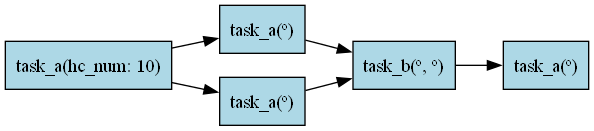
\includegraphics[width=\columnwidth]{Images/mine/dag_lang_example.png}
    \caption{Simple DAG example}
    \label{fig:dag_lang_example}
\end{figure}

When \texttt{task\_a(10)} is invoked, it doesn't actually run the user code. It instead creates a representation of the task, which can be passed as argument to other tasks. The workflow planning and execution only happens once \texttt{.compute()} is called on the last/sink task (\texttt{a4}), as shown in Listing~\ref{lst:setup_and_launch_workflow_execution}. When \texttt{compute()} is called, we can create a representation of the entire workflow structure by backtracking the task dependencies.

\begin{figure}[h]
\centering
\begin{lstlisting}[language=Python, basicstyle=\ttfamily\footnotesize, columns=fullflexible, breaklines=true]
result = a4.compute(
    dag_name="simpledag", 
    config=Worker.Config(
        faas_gateway_address=...,
        intermediate_storage_config=(ip, port, password),
        metrics_storage_config=(ip, port, password),
        planner_config=UniformPlanner.Config(
            sla=sla,
            worker_resource_configuration=TaskWorkerResourceConfiguration(cpus=3, memory_mb=512),
            optimizations=[PreLoadOptimization, TaskDupOptimization]
        )
    )
)
\end{lstlisting}
\caption{Setting up and launching workflow execution}
\label{lst:setup_and_launch_workflow_execution}
\end{figure}

One limitation of this DAG definition language is that it doesn't support "dynamic fan-outs" (e.g., creating a variable number of tasks depending on the result of another task) on a single workflow. This is a powerful and expressive feature, but that is seldom supported in other DAG definition languages (e.g., Dask, WUKONG, Unum, Oozie~\cite{apache_oozie} do not support it). These languages require the user to split the workflow into multiple workflows, one for each \textit{dynamic fan-out}: one workflow runs up to the task that generates a list of results, while a second workflow starts with a number of tasks that depends on the size or contents of that list. 

Apache AirFlow~\footnote{https://airflow.apache.org/docs/apache-airflow/stable/authoring-and-scheduling/dynamic-task-mapping.html} supports this feature through an extension to their DAG language, allowing a variable number of tasks to be created at run-time depending on the number of results produced by a previous task. Implementing similar functionality is possible, but it would reduce the accuracy of predictions. This is because we would also need to predict the expected fan-out size, and any errors in that prediction could amplify inaccuracies in the predictions for the rest of the workflow.

We will now present the architecture, highlighting the core layers of our solution.

% #############################################################################
\section{Overview}
The overall architecture and logical flow of our decentralized serverless workflow execution engine is organized into 3 high-level layers. Figure~\ref{fig:solution_architecture} provides an overview of this architecture. The upper part represents the components that run on the user's machine, while the lower part represents the components that run outside the user's machine. 

The user writes its workflows in Python (demonstrated in Section \ref{ss:workflow_definition_language}). First, a planning algorithm, chosen by the user, will run locally to generate a static workflow plan. This plan defines a task-to-worker mapping and other task-level optimization hints for FaaS workers. Once the plan is done, the client launches the initial workers for the root tasks, kicking off workflow execution. The user program then waits for a storage notification indicating workflow completion and then retrieves the final result from storage.

The following sections should provide a deeper understanding of each layer as well as how the user interacts with the system.

\begin{figure}[h]
  \centering
  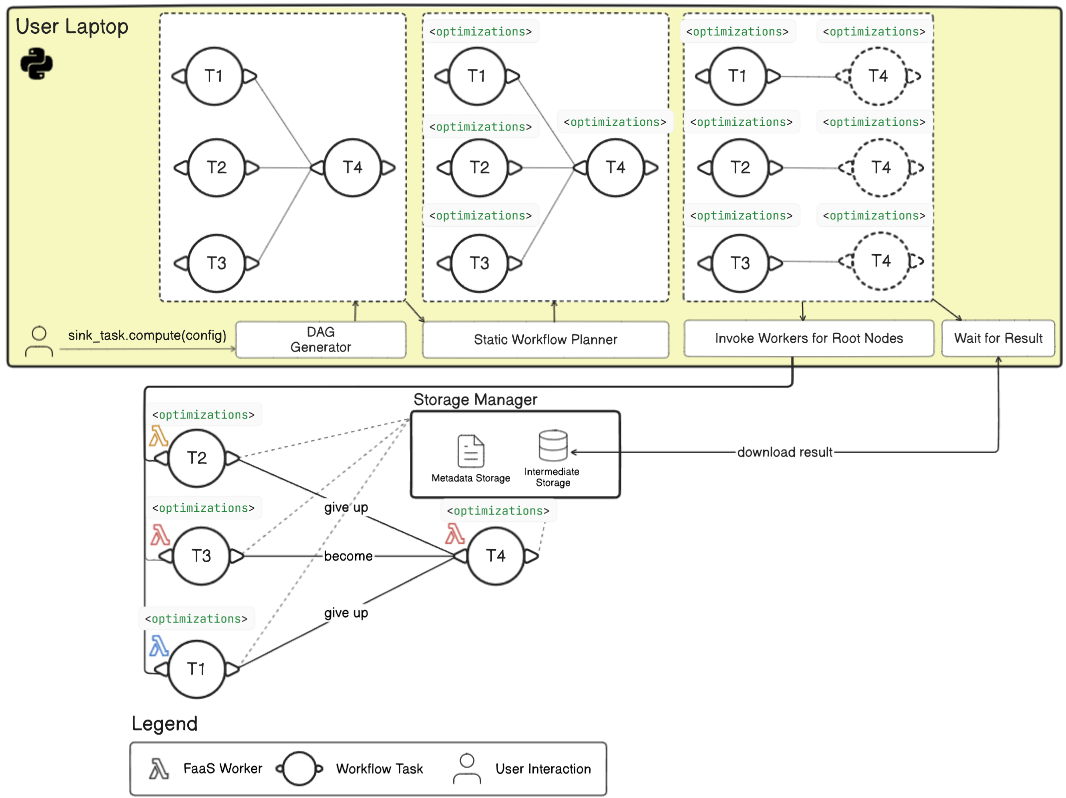
\includegraphics[width=\columnwidth]{Images/mine/solution_distributedarchintegrated.png}
  \caption{Solution Architecture}
  \label{fig:solution_architecture}
\end{figure}

\begin{enumerate}
    \item \textbf{Metadata Management}: Responsible for collecting and storing task metadata from previous executions. It also uses this metadata to provide predictions regarding task execution times, data transfer times, task output sizes, and worker startup times;
    \item \textbf{Static Workflow Planning}: Receives the entire workflow, represented as a Directed Acyclic Graph (DAG), and a "planner" (an algorithm chosen by the user). This planner will use the predictions provided by Metadata Management to create a static plan/schedule to be followed by the workers;
    \item \textbf{Scheduling}: This component is integrated into the workers, and it is responsible for executing the plan generated by the Static Workflow Planning layer, applying optimizations and delegating tasks as needed.
\end{enumerate}

There are 3 distinct computational entities involved in this system:

\begin{itemize}
    \item \textbf{User Computer}: Responsible for creating workflow plans, submitting them (triggering workflow execution), and receiving its results. The planning phase also happens on this computer, right before a workflow is submitted for execution;
    \item \textbf{Workers}: These are the FaaS workers (often running in containerized environments), that execute one or more tasks. The decentralization of our solution is due to the fact that these workers are responsible for scheduling of subsequent tasks, delegating tasks and launching new workers when needed without requiring a central scheduler. Lastly, they are also responsible for collecting and uploading metadata;
    \item \textbf{Storage}: Consists of an \textit{Intermediate Storage} for intermediate outputs which may be needed for subsequent tasks and a \textit{Metadata Storage} for information crucial to workflow execution (e.g., notifications about task readiness and completion).
\end{itemize}

Next, we will explain how the user defines and submits workflows for execution.
% #############################################################################
\section{Metadata Management}
\label{ss:metadata_management}
The goal of the \textbf{Metadata Management} layer is to provide the most accurate task-wise predictions to help the planner algorithm chosen by the user to make better decisions. To achieve this, while the workflow is running we collect metrics about each task's execution. These metrics are stored in \textit{Metadata Storage}: task execution time, data transfer size and time, task input and output sizes, and worker startup time. 

Storing these metrics enables us to provide a prediction API, shown in Listing~\ref{lst:task_predictions_api}. To improve accuracy, metrics are kept separate for each workflow. As a result, even if two workflows use the same function or task code, their metrics are stored independently. This design choice reflects our assumption that different workflows may follow different execution patterns. To avoid introducing runtime overhead, metrics are batched and uploaded when the worker shuts down.

The prediction methods take an additional parameter, \texttt{SLA} (Service-level Agreement), which is specified by the user and influences the selection of prediction samples. For example, \texttt{SLA="median"} will use the median of the historical samples, whereas \texttt{SLA=Percentile(80)} will return a more conservative estimate. By allowing the user to control this parameter, the API can provide predictions that are tailored to different performance requirements.

\begin{figure}[h]
\centering
\begin{lstlisting}[basicstyle=\ttfamily\footnotesize, columns=fullflexible, breaklines=true]
class PredictionsProvider:
  def predict_output_size(function_name, input_size, sla) -> int

  def predict_worker_startup_time(resource_config, state: 'cold' | 'warm', sla) -> float

  def predict_data_transfer_time(
        type: 'upload' | 'download',
        data_size_bytes,
        resource_config,
        sla
    ) -> float

  def predict_execution_time(
        task_name,
        input_size,
        resource_config,
        sla: SLA
    ) -> float
\end{lstlisting}
\caption{Task Predictions API}
\label{lst:task_predictions_api}
\end{figure}

In addition, metrics such as worker startup time, data transfer time, and task execution time are tied to the specific worker resource configuration. To account for this, our prediction method follows two paths. If we have enough historical samples for the same resource configuration, we use only those. Otherwise, when there are not enough samples with the same resource configuration, we fall back to a normalization strategy: we adjust samples from other memory configurations to a baseline, use those to estimate execution time, and then rescale the result back to the target configuration. 

After filtering samples we use an algorithm that selects a limited number of the most relevant samples for each prediction. This algorithm works by gradually widening a tolerance window around the reference value until it finds enough nearby samples. Within each window, it balances samples that are smaller, larger, or exactly equal to the reference, giving preference to the closest ones. If there still aren't enough candidates, it falls back to simply picking the nearest available samples overall. This way, the algorithm adapts to the data while keeping the selection both relevant and limited in size.


% #############################################################################
\section{Static Workflow Planning}

\subsection{Simulation Layer}
% TODO: Metrics collected, how predictions are done/cached to be faster

\subsection{Planning Algorithms}

This layer executes on the user side, and it receives the workflow representation and a workflow planning algorithm chosen by the user (as shown in Listing \ref{lst:setup_and_launch_workflow_execution}). Its job is to execute the planning algorithm, providing it access to the predictions exposed by the Metadata Management layer (Section \ref{ss:metadata_management}).

Planners can run \textit{workflow simulations} based on the predictions, allowing them to experiment with different resource configurations for different tasks and different task co-location strategies. Additionally, they can apply different user-selected optimizations. The accuracy of these simulations depends on the accuracy of the predictions exposed by the \textit{Predictions API}.

For each task, the planner assigns both a \texttt{worker\_id} and a resource configuration (vCPUs and memory). The \texttt{worker\_id} specifies the worker instance that must execute the task—analogous to the “colors” in Palette Load Balancing~\cite{palette_load_balancing}, but in our case this assignment is mandatory rather than advisory, giving strict control over execution locality. Two tasks assigned the same \texttt{worker\_id} should be executed on the same worker instance. If \texttt{worker\_id} is not specified, workers will, at run-time, have to decide whether to execute or delegate those tasks, similar to WUKONG's ~\cite{wukong_2} scheduling. We refer to these workers as \textit{"flexible workers"}.

Users can select from three provided planners or implement their own planner by implementing an interface. All planners have access to the predictions API as well as the workflow simulation. The planners the user can choose from are the following:

\begin{enumerate}
    \item \textbf{WUKONG}: All tasks will use the same worker configuration (specified by the user) and won't be assigned a \texttt{worker\_id}, meaning they will be executed by \textit{"flexible workers"}. This is a more dynamic scheduling approach where tasks aren't tied to specific workers that try to reproduce WUKONG's scheduling behavior;
    \item \textbf{Uniform}: Tasks share a common worker configuration specified by the user, with each task assigned a \texttt{worker\_id} to allow for co-location of tasks.
    \item \textbf{Non-Uniform}: Tasks can use different worker configurations (list of available resources is specified by the user). Each task is assigned a \texttt{worker\_id}. This algorithm starts by assigning the best available resources to all tasks. Then it runs a resource downgrading algorithm that attempts to downgrade resources of workers \textit{outside the critical path} as much as possible without introducing a new critical path.
\end{enumerate}

Both the \textbf{Uniform} and \textbf{Non-Uniform} planners follow a two-phase approach for task allocation: resource configuration assignment followed by worker ID assignment. The planners differ in their resource allocation strategies. The \textbf{Uniform planner} applies a single, user-specified CPU and memory configuration to all tasks, while the \textbf{Non-Uniform planner} selects the most powerful configuration from the user-specified options for each task. After resource configuration, both planners employ the logic detailed in Algorithm \ref{alg:worker_assignment} for worker ID assignment. This algorithm implements an intelligent clustering strategy with two primary objectives: launch as few new workers as possible while trying not to overload workers; and minimizing network data transfers by co-locating tasks whose outputs are expected to be larger. This clustering approach provides an additional benefit of reducing fan-in operation costs.

\begin{algorithm}
    \caption{Worker Assignment Algorithm}
    \label{alg:worker_assignment}
    \small
    \begin{algorithmic}[1]
    \Require $nodes$, $predictions$, $base\_rc$, $SLA$, $MAX\_CLUSTERING$
    \State $assigned \gets \emptyset$
    
    \Comment{nodes are topologically sorted}
    \ForAll{$n \in nodes$}
        \If{$n \in assigned$}
            \State \textbf{continue}
        \EndIf
        
        \If{$n.upstream = \emptyset$} \Comment{root nodes}
            \State $roots \gets \{r \in nodes \mid r.upstream = \emptyset \land r \notin assigned\}$
            \State \Call{AssignGroup}{$\textit{null}$, $roots$}
        \ElsIf{$|n.upstream| = 1$} \Comment{1$\to$1 or 1$\to$N}
            \State $u \gets n.upstream[0]$
            \If{$|u.downstream| = 1$}
                \State \Call{AssignWorker}{$[n]$, $u.worker$} \Comment{reuse worker}
            \Else \Comment{1$\to$N}
                \State $fanout \gets \{d \in u.downstream \mid d \notin assigned\}$
                \State \Call{AssignGroup}{$u.worker$, $fanout$}
            \EndIf
        \Else \Comment{N$\to$1}
            \State $outputs \gets \{u.worker: predictions.output\_size(u) \mid u \in n.upstream\}$
            \State $best \gets \arg\max_{w \in outputs} outputs[w]$
            \State \Call{AssignWorker}{$[n]$, $best$}
        \EndIf
    \EndFor
    
    \Statex
    
    \Function{AssignGroup}{$up\_worker$, $tasks$}
        \If{$tasks = \emptyset$}
            \Return
        \EndIf
        
        \State $exec\_t \gets \{t: predictions.exec\_time(t) \mid t \in tasks\}$
        \State $out\_sz \gets \{t: predictions.output\_size(t) \mid t \in tasks\}$
        \State $median \gets \textsc{Median}(exec\_t.values())$
        \State $longs \gets \{t \in tasks \mid exec\_t[t] > median\}$
        \State $shorts \gets \textsc{SortLargerOutputFirst}(\{t \in tasks \mid exec\_t[t] \leq median\})$
        
        \Statex
        \State \Comment{1) cluster short tasks with bigger outputs on upstream worker}
        \If{$up\_worker \neq \textit{null} \land shorts \neq \emptyset$}
            \State $cluster \gets shorts[0:MAX\_CLUSTERING]$
            \State \Call{AssignWorker}{$cluster$, $up\_worker$}
            \State $shorts \gets shorts[MAX\_CLUSTERING:]$
        \EndIf
        
        \Statex
        \State \Comment{2) pair long tasks with remaining short tasks (1 long per group)}
        \While{$longs \neq \emptyset \land shorts \neq \emptyset$}
            \State $cluster \gets [longs[0]] + shorts[0:MAX\_CLUSTERING-1]$
            \State $worker\_id \gets$ \Call{NewWorkerId}{}
            \State \Call{AssignWorker}{$cluster$, $worker\_id$}
            \State $longs \gets longs[1:]$
            \State $shorts \gets shorts[MAX\_CLUSTERING-1:]$
        \EndWhile
        
        \Statex
        \State \Comment{3) group remaining short tasks}
        \While{$shorts \neq \emptyset$}
            \State $worker\_id \gets$ \Call{NewWorkerId}{}
            \State \Call{AssignWorker}{$shorts[0:MAX\_CLUSTERING]$, $worker\_id$}
            \State $shorts \gets shorts[MAX\_CLUSTERING:]$
        \EndWhile
        
        \Statex
        \State \Comment{4) group remaining longs (half-size)}
        \State $half \gets \max(1, \lfloor MAX\_CLUSTERING / 2 \rfloor)$
        \While{$longs \neq \emptyset$}
            \State $worker\_id \gets$ \Call{NewWorkerId}{}
            \State \Call{AssignWorker}{$longs[0:half]$, $worker\_id$}
            \State $longs \gets longs[half:]$
        \EndWhile
    \EndFunction
\end{algorithmic}
\end{algorithm}


After this, the \textbf{Non-Uniform} planner runs an additional algorithm, shown in Algorithm \ref{alg:resource_downgrading}, that attempts to downgrade resources of workers \textit{outside the critical path} as much as possible without introducing a new critical path, by iteratively simulating the effect of downgrading resources of workers \textit{outside the critical path} with different configurations.

\begin{algorithm}
    \caption{Resource Downgrading Algorithm}
    \label{alg:resource_downgrading}
    \small
    \begin{algorithmic}[1]
    \Require $dag$, $nodes$, $critical\_path\_ids$, $original\_cp\_time$, $configs$, $predictions$
    \State $workers\_outside \gets \emptyset$
    
    \Statex
    \State \Comment{1) Identify workers outside the critical path}
    \ForAll{$n \in nodes$} \Comment{nodes are topologically sorted}
        \State $wid \gets n.worker\_id$
        \If{$n.id \notin critical\_path\_ids \land \forall cp \in dag.critical\_path\_nodes: wid \neq cp.worker\_id$}
            \State $workers\_outside \gets workers\_outside \cup \{wid\}$
        \EndIf
    \EndFor
    
    \State $nodes\_outside\_cp \gets \{n \in nodes \mid n.id \notin critical\_path\_ids\}$
    
    \Statex
    \State \Comment{2) Attempt downgrade for each worker outside critical path}
    \ForAll{$wid \in workers\_outside$}
        \State $last\_good_\_rc \gets \{n.id: n.config \mid n \in nodes\_outside\_cp \land n.worker\_id = wid\}$
        
        \Statex
        \State \Comment{Iterate through weaker configurations (skip strongest at index 0)}
        \For{$i \gets 1$ \textbf{to} $|configs| - 1$}
            \State $trial \gets configs[i].\textsc{Clone}(wid)$
            
            \Statex
            \State \Comment{Apply trial configuration to all nodes of this worker}
            \ForAll{$n \in nodes\_outside\_cp$}
                \If{$n.worker\_id = wid$}
                    \State $n.config \gets trial$
                \EndIf
            \EndFor
            
            \Statex
            \State \Comment{Recompute workflow timing with predictions}
            \State $cp\_time \gets$ \Call{SimulateCriticalPathTime}{$dag$}
            
            \Statex
            \If{$cp\_time = original\_cp\_time$}
                \State \Comment{Downgrade acceptable, record as last good state}
                \ForAll{$n \in nodes\_outside\_cp$}
                    \If{$n.worker\_id = wid$}
                        \State $last\_good\_rc[n.id] \gets n.config$
                    \EndIf
                \EndFor
            \Else
                \State \Comment{Downgrade increases critical path, revert and move on to the next worker}
                \ForAll{$n \in nodes\_outside\_cp$}
                    \If{$n.worker\_id = wid$}
                        \State $n.config \gets last\_good\_rc[n.id]$
                    \EndIf
                \EndFor
                \State \textbf{break} \Comment{move to next worker}
            \EndIf
        \EndFor
    \EndFor
    
\end{algorithmic}
\end{algorithm}


With the information they have access to, planners can estimate whether it is worthwhile to offload a task to a more powerful worker. This involves weighing the overhead of uploading the input data, waiting for the worker to be provisioned, and then executing the task, against the alternative of simply executing the task on the current, less powerful worker.

\subsection{Optimizations}

Aside from their \texttt{worker\_id} and resource assignments, planners can also apply different \textbf{optimizations} to further improve the workflow execution. The optimizations to be used are selected by the user, as shown in Listing \ref{lst:setup_and_launch_workflow_execution}. Similarly to planners, we provide three optimizations: \textbf{pre-warm}, \textbf{pre-load} and \textbf{task-dup}, but it is also possible to create new optimizations and define how workers should react to them. Now, we will describe the three base optimizations and how they are assigned to tasks:

\begin{enumerate}
\item\textbf{pre-warm}(worker\_config) [Pre-warming Workers]:
\begin{itemize}
  \item \textit{Interpretation}: Tasks/Nodes with this optimization should perform a special invocation to the FaaS gateway that forces it to launch a new worker with the specified resource configuration \texttt{worker\_config}. This can be used to warm up workers ahead of time and mask cold start latencies;
  \item \textit{Assignment Logic}: For the nodes whose workers are expected to have cold starts, find the "optimal" node to perform the pre-warming by searching for nodes/tasks whose activity timing falls within a window (goal: avoid the pre-warmed worker from going cold before needed, while also not being warm too late). The optimization will be added to the "optimal" node, which will be responsible for doing the special "empty invocation" to the FaaS gateway.
\end{itemize}

\item\textbf{pre-load} [Pre-Loading Dependencies]:
\begin{itemize}
  \item \textit{Interpretation}: Workers assigned to tasks or nodes with this optimization should begin downloading the task's dependencies as early as possible. This prevents scenarios where a worker must fetch all dependencies at once. The optimization is effective only if the worker is active before executing the task, allowing it to download dependencies in parallel with other ongoing tasks. This is implemented by having the worker receive completion notifications from the \textit{Metadata Storage} for all tasks upstream of the optimized task;
  \item \textit{Assignment Logic}: First, all tasks with more than a configurable threshold of dependencies/upstream tasks are assigned the optimization. Then, an iterative process is used to optimize the workflow along its critical path using this optimization. First, the algorithm identifies the critical path and assigns the optimization to eligible nodes on it. The critical path is then recalculated: if the total execution time increases, the optimization is removed; if the execution time decreases but the critical path changes, the algorithm restarts with the new path. This process repeats until no further improvements are possible, or the algorithm hits a fixed iteration limit.
\end{itemize}

\item\textbf{task-dup} [Task Duplication]:
\begin{itemize}
  \item \textit{Interpretation}: Tasks or nodes with this optimization can be executed by other workers if doing so helps unlock dependent tasks more quickly. The task could be "duplicated" by workers that depend on its output. It is a trade-off between performance and resource utilization, allowing potentially faster execution at the cost of using additional compute resources;
  \item \textit{Assignment Logic}: Assigned to all nodes whose execution time and input size do not exceed predefined thresholds. Whether duplication actually occurs is decided at run-time. The optimization targets fast tasks with small inputs, as these are inexpensive to duplicate in terms of both downloading dependencies and execution. This way, even if duplication turns out to be unnecessary, the impact on performance and resource usage remains minimal.
\end{itemize}
\end{enumerate}
Because planners may sometimes lack sufficient information to make optimal decisions about optimization assignments, it is important to not only allow the user to select optimizations at the workflow-level, but also allow them the flexibility to specify optimizations at the \textit{task-level}. An example of this feature is shown in Listing~\ref{lst:dag_lang_example}, where the user requests that \texttt{task\_b} attempt to use the \textit{pre-load} optimization.

Once these optimizations are assigned, workflow planning is complete, and workers can begin execution. Because planning occurs on the user's machine (i.e., the machine launching the workflow), it is responsible for initiating the workflow by starting the initial workers. From that point onward, workers dynamically invoke additional workers as needed, following a choreographed, decentralized execution model.

\begin{figure*}[h]
    \centering
    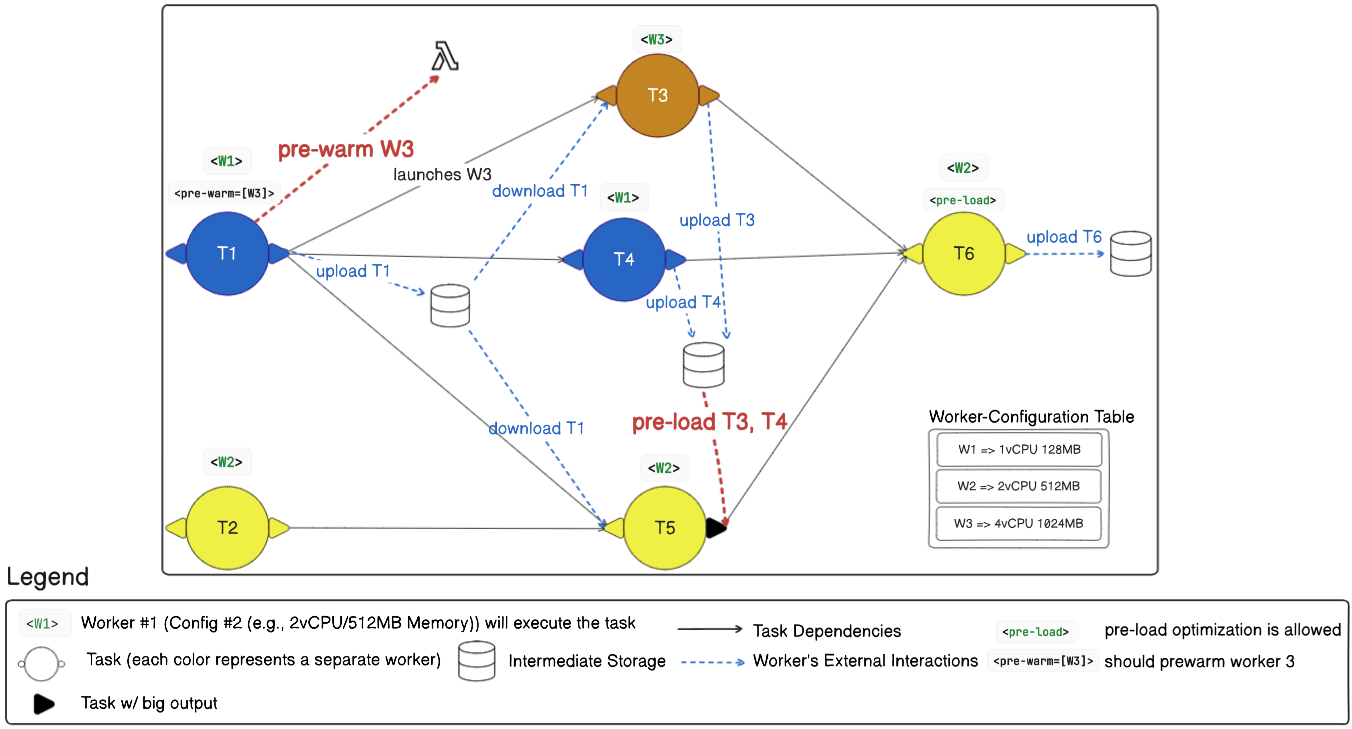
\includegraphics[width=\textwidth]{Images/mine/solution_workflowinstanceexample.png}
    \caption{Planned Workflow Execution Example}
    \label{fig:planned_workflow_execution_example}
\end{figure*}

To illustrate this execution model, Figure~\ref{fig:planned_workflow_execution_example} provides a visual trace of how a planned workflow would be executed. The diagram depicts the workflow with the optimizations and \texttt{worker\_id} assignments for each task. The non-dashed arrows represent task dependencies, while the dashed arrows represent interactions with the \textit{Intermediate Storage} to either upload or download task data. We can see that task outputs are only uploaded to storage when there is at least one downstream task that depends on it and is assigned to another worker. 

It is also worth noting that the planner assigned \texttt{Task 6} to \texttt{Worker 2}. This decision might be due to \texttt{Worker 2} being more powerful than \texttt{Worker 1}, and because the output of \texttt{Task 5} is larger than that of \texttt{Tasks 4} and \texttt{5}. Therefore, even if the task were executed on a more powerful worker (such as \texttt{Worker 3}, which handled \texttt{Task 3}), the potential performance gain would not offset the additional time or resources required. This is an example of a planner deciding to co-locate \texttt{Tasks 5 and 6} on the same worker to reduce data movement.

Regarding \textbf{optimizations}, we can see \texttt{Task 1} \texttt{pre-warming} \texttt{Worker 3}, by making  a dummy invocation to the FaaS gateway, in an attempt to make it available before \texttt{Task 3} needs it. The \texttt{pre-load} optimization is used in \texttt{Task 5}, where the planner decided that \texttt{Worker 2} should start downloading the external dependencies for \texttt{Task 6} (\texttt{Task 3} and \texttt{Task 4}) as soon as they are available. This \texttt{pre-loading} can begin as soon as \texttt{Task 6}'s dependencies are ready in storage, potentially overlapping with \texttt{Task 2}'s execution instead of \texttt{Task 5}, as shown in the figure.

\begin{algorithm}
    \caption{Worker Assignment Algorithm}
    \label{alg:worker_assignment}
    \small
    \begin{algorithmic}[1]
    \Require $nodes$, $predictions$, $base\_rc$, $SLA$, $MAX\_CLUSTERING$
    \State $assigned \gets \emptyset$
    
    \Comment{nodes are topologically sorted}
    \ForAll{$n \in nodes$}
        \If{$n \in assigned$}
            \State \textbf{continue}
        \EndIf
        
        \If{$n.upstream = \emptyset$} \Comment{root nodes}
            \State $roots \gets \{r \in nodes \mid r.upstream = \emptyset \land r \notin assigned\}$
            \State \Call{AssignGroup}{$\textit{null}$, $roots$}
        \ElsIf{$|n.upstream| = 1$} \Comment{1$\to$1 or 1$\to$N}
            \State $u \gets n.upstream[0]$
            \If{$|u.downstream| = 1$}
                \State \Call{AssignWorker}{$[n]$, $u.worker$} \Comment{reuse worker}
            \Else \Comment{1$\to$N}
                \State $fanout \gets \{d \in u.downstream \mid d \notin assigned\}$
                \State \Call{AssignGroup}{$u.worker$, $fanout$}
            \EndIf
        \Else \Comment{N$\to$1}
            \State $outputs \gets \{u.worker: predictions.output\_size(u) \mid u \in n.upstream\}$
            \State $best \gets \arg\max_{w \in outputs} outputs[w]$
            \State \Call{AssignWorker}{$[n]$, $best$}
        \EndIf
    \EndFor
    
    \Statex
    
    \Function{AssignGroup}{$up\_worker$, $tasks$}
        \If{$tasks = \emptyset$}
            \Return
        \EndIf
        
        \State $exec\_t \gets \{t: predictions.exec\_time(t) \mid t \in tasks\}$
        \State $out\_sz \gets \{t: predictions.output\_size(t) \mid t \in tasks\}$
        \State $median \gets \textsc{Median}(exec\_t.values())$
        \State $longs \gets \{t \in tasks \mid exec\_t[t] > median\}$
        \State $shorts \gets \textsc{SortLargerOutputFirst}(\{t \in tasks \mid exec\_t[t] \leq median\})$
        
        \Statex
        \State \Comment{1) cluster short tasks with bigger outputs on upstream worker}
        \If{$up\_worker \neq \textit{null} \land shorts \neq \emptyset$}
            \State $cluster \gets shorts[0:MAX\_CLUSTERING]$
            \State \Call{AssignWorker}{$cluster$, $up\_worker$}
            \State $shorts \gets shorts[MAX\_CLUSTERING:]$
        \EndIf
        
        \Statex
        \State \Comment{2) pair long tasks with remaining short tasks (1 long per group)}
        \While{$longs \neq \emptyset \land shorts \neq \emptyset$}
            \State $cluster \gets [longs[0]] + shorts[0:MAX\_CLUSTERING-1]$
            \State $worker\_id \gets$ \Call{NewWorkerId}{}
            \State \Call{AssignWorker}{$cluster$, $worker\_id$}
            \State $longs \gets longs[1:]$
            \State $shorts \gets shorts[MAX\_CLUSTERING-1:]$
        \EndWhile
        
        \Statex
        \State \Comment{3) group remaining short tasks}
        \While{$shorts \neq \emptyset$}
            \State $worker\_id \gets$ \Call{NewWorkerId}{}
            \State \Call{AssignWorker}{$shorts[0:MAX\_CLUSTERING]$, $worker\_id$}
            \State $shorts \gets shorts[MAX\_CLUSTERING:]$
        \EndWhile
        
        \Statex
        \State \Comment{4) group remaining longs (half-size)}
        \State $half \gets \max(1, \lfloor MAX\_CLUSTERING / 2 \rfloor)$
        \While{$longs \neq \emptyset$}
            \State $worker\_id \gets$ \Call{NewWorkerId}{}
            \State \Call{AssignWorker}{$longs[0:half]$, $worker\_id$}
            \State $longs \gets longs[half:]$
        \EndWhile
    \EndFunction
\end{algorithmic}
\end{algorithm}

\begin{algorithm}
    \caption{Resource Downgrading Algorithm}
    \label{alg:resource_downgrading}
    \small
    \begin{algorithmic}[1]
    \Require $dag$, $nodes$, $critical\_path\_ids$, $original\_cp\_time$, $configs$, $predictions$
    \State $workers\_outside \gets \emptyset$
    
    \Statex
    \State \Comment{1) Identify workers outside the critical path}
    \ForAll{$n \in nodes$} \Comment{nodes are topologically sorted}
        \State $wid \gets n.worker\_id$
        \If{$n.id \notin critical\_path\_ids \land \forall cp \in dag.critical\_path\_nodes: wid \neq cp.worker\_id$}
            \State $workers\_outside \gets workers\_outside \cup \{wid\}$
        \EndIf
    \EndFor
    
    \State $nodes\_outside\_cp \gets \{n \in nodes \mid n.id \notin critical\_path\_ids\}$
    
    \Statex
    \State \Comment{2) Attempt downgrade for each worker outside critical path}
    \ForAll{$wid \in workers\_outside$}
        \State $last\_good_\_rc \gets \{n.id: n.config \mid n \in nodes\_outside\_cp \land n.worker\_id = wid\}$
        
        \Statex
        \State \Comment{Iterate through weaker configurations (skip strongest at index 0)}
        \For{$i \gets 1$ \textbf{to} $|configs| - 1$}
            \State $trial \gets configs[i].\textsc{Clone}(wid)$
            
            \Statex
            \State \Comment{Apply trial configuration to all nodes of this worker}
            \ForAll{$n \in nodes\_outside\_cp$}
                \If{$n.worker\_id = wid$}
                    \State $n.config \gets trial$
                \EndIf
            \EndFor
            
            \Statex
            \State \Comment{Recompute workflow timing with predictions}
            \State $cp\_time \gets$ \Call{SimulateCriticalPathTime}{$dag$}
            
            \Statex
            \If{$cp\_time = original\_cp\_time$}
                \State \Comment{Downgrade acceptable, record as last good state}
                \ForAll{$n \in nodes\_outside\_cp$}
                    \If{$n.worker\_id = wid$}
                        \State $last\_good\_rc[n.id] \gets n.config$
                    \EndIf
                \EndFor
            \Else
                \State \Comment{Downgrade increases critical path, revert and move on to the next worker}
                \ForAll{$n \in nodes\_outside\_cp$}
                    \If{$n.worker\_id = wid$}
                        \State $n.config \gets last\_good\_rc[n.id]$
                    \EndIf
                \EndFor
                \State \textbf{break} \Comment{move to next worker}
            \EndIf
        \EndFor
    \EndFor
    
\end{algorithmic}
\end{algorithm}


% #############################################################################

\section{Decentralized Scheduling}

Since our target execution platform is FaaS, the worker logic is implemented as a FaaS handler. Due to the decentralized nature of our solution, workers will be responsible for performing both task execution and scheduling in a choreographed manner. 

When invoked, a worker receives the \texttt{workflow\_id} and the \texttt{task\_ids} of the tasks it should execute first. Using this information, it retrieves the DAG structure and execution plan from \textit{Metadata Storage}. Rather than immediately executing the initial tasks, the worker first subscribes to \texttt{TASK\_READY} and \texttt{TASK\_COMPLETED} events for specific tasks. These events are essential both for enabling certain optimizations and for ensuring the worker follows the workflow plan correctly.

After that, the worker starts executing the initial tasks concurrently. The logic for executing tasks is the following:
\begin{enumerate}
    \item \textbf{Gathering Dependencies}: Check which dependencies are missing (not downloaded yet) and download them from storage;
    \item \textbf{Executing Task}: Execute the task. Tasks' code is stored in a serialized/pickled format (using cloudpickle\footnote{https://github.com/cloudpipe/cloudpickle}) and deserialized and executed by the workers. This enables the worker to remain generic, capable of receiving and executing arbitrary task code;
    \item \textbf{Handling Output}: This phase is responsible for evaluating whether it's necessary to upload the task's output to storage and emitting a \texttt{TASK\_COMPLETED} event;
    \item \textbf{Delegating Downstream Tasks}: For each downstream task, the worker performs an \texttt{atomic\_increment\_and\_get()} operation on a "dependency counter" (inspired by WUKONG~\cite{wukong_2}) stored in \textit{Metadata Storage}, which tracks how many dependencies of a task have been satisfied. When the counter indicates that all dependencies for a downstream task have been satisfied, the worker emits a \texttt{TASK\_READY} event for that task. The worker then consults the execution plan to determine how to proceed for each downstream task unlocked: if the unlocked task is assigned to another worker, a \texttt{TASK\_READY} event is emitted; if the unlocked task is assigned to the same worker and has no remaining dependencies, the worker immediately continues the cycle by executing it.
\end{enumerate}

To illustrate how workers handle downstream tasks, Figure~\ref{fig:choreographed_scheduling_example} presents an example of choreographed decentralized scheduling with three workers (A, B, and C) and seven tasks (T1-T7). In this example, once Task T1 completes on Worker B, the worker inspects the dependency counters for tasks T3, T4, and T5. It determines that T3 and T4 are ready to run, while T5 is still pending because Task T2 has not yet completed. Worker B then launches a new worker (C) to execute T3 and proceeds to execute T4 itself. Later, when T2 finishes on Worker A, all dependencies of T5 are satisfied, prompting Worker A to execute it directly.

\begin{figure}[h]
    \centering
    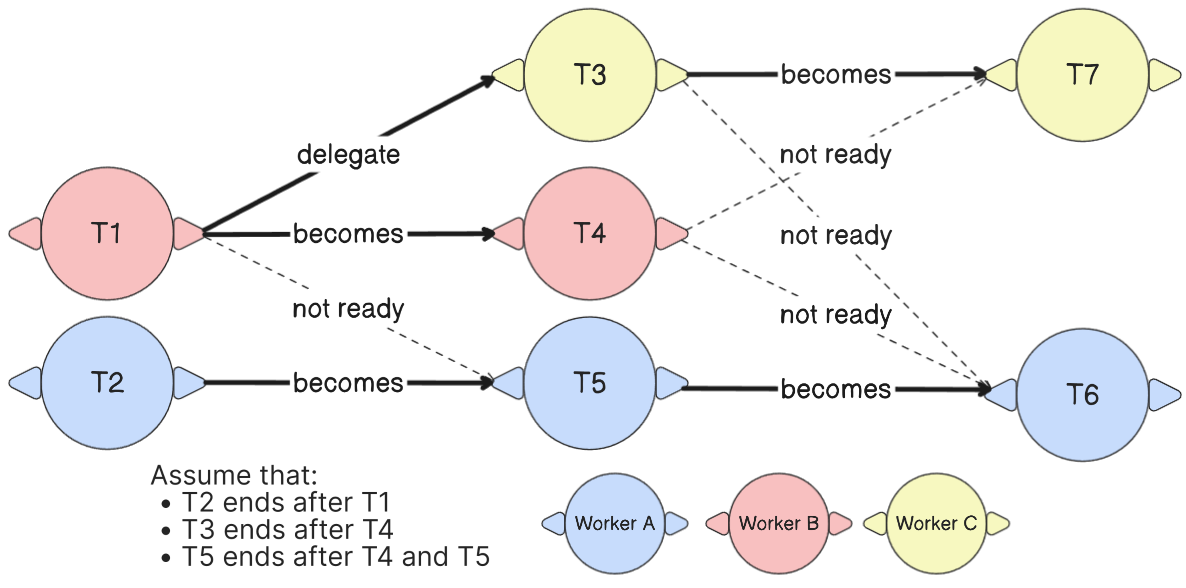
\includegraphics[width=0.5\textwidth]{Images/mine/choreographed_execution_example.png}
    \caption{Choreographed Scheduling Example}
    \label{fig:choreographed_scheduling_example}
\end{figure}

A workflow is considered complete once the output of the final (sink) task is available in storage. The worker that uploads this final result is also responsible for cleaning up all intermediate results before shutting down. Meanwhile, after submitting the workflow, the user's machine subscribes to the \texttt{TASK\_COMPLETED} event for the sink task; upon receiving this notification, it retrieves the final result from \textit{Intermediate Storage}.

By delegating downstream tasks to workers, our approach eliminates the need for a central scheduler, a common component in many existing FaaS-based workflow engines. This decentralization increases flexibility and scalability, as workers can dynamically invoke additional workers as needed, following a choreographed decentralized execution model.

Having described the design and implementation of the system, we now turn to its evaluation. The next section presents the experimental setup, results, and analysis used to assess the strengths and weaknesses of our approach.